% Auto-generated figure blocks for the paper. \graphicspath{{paper_figures/}}
% Each montage = labelled floor plan (left) + coloured 3D render (right).

\begin{figure}[t]
  \centering
  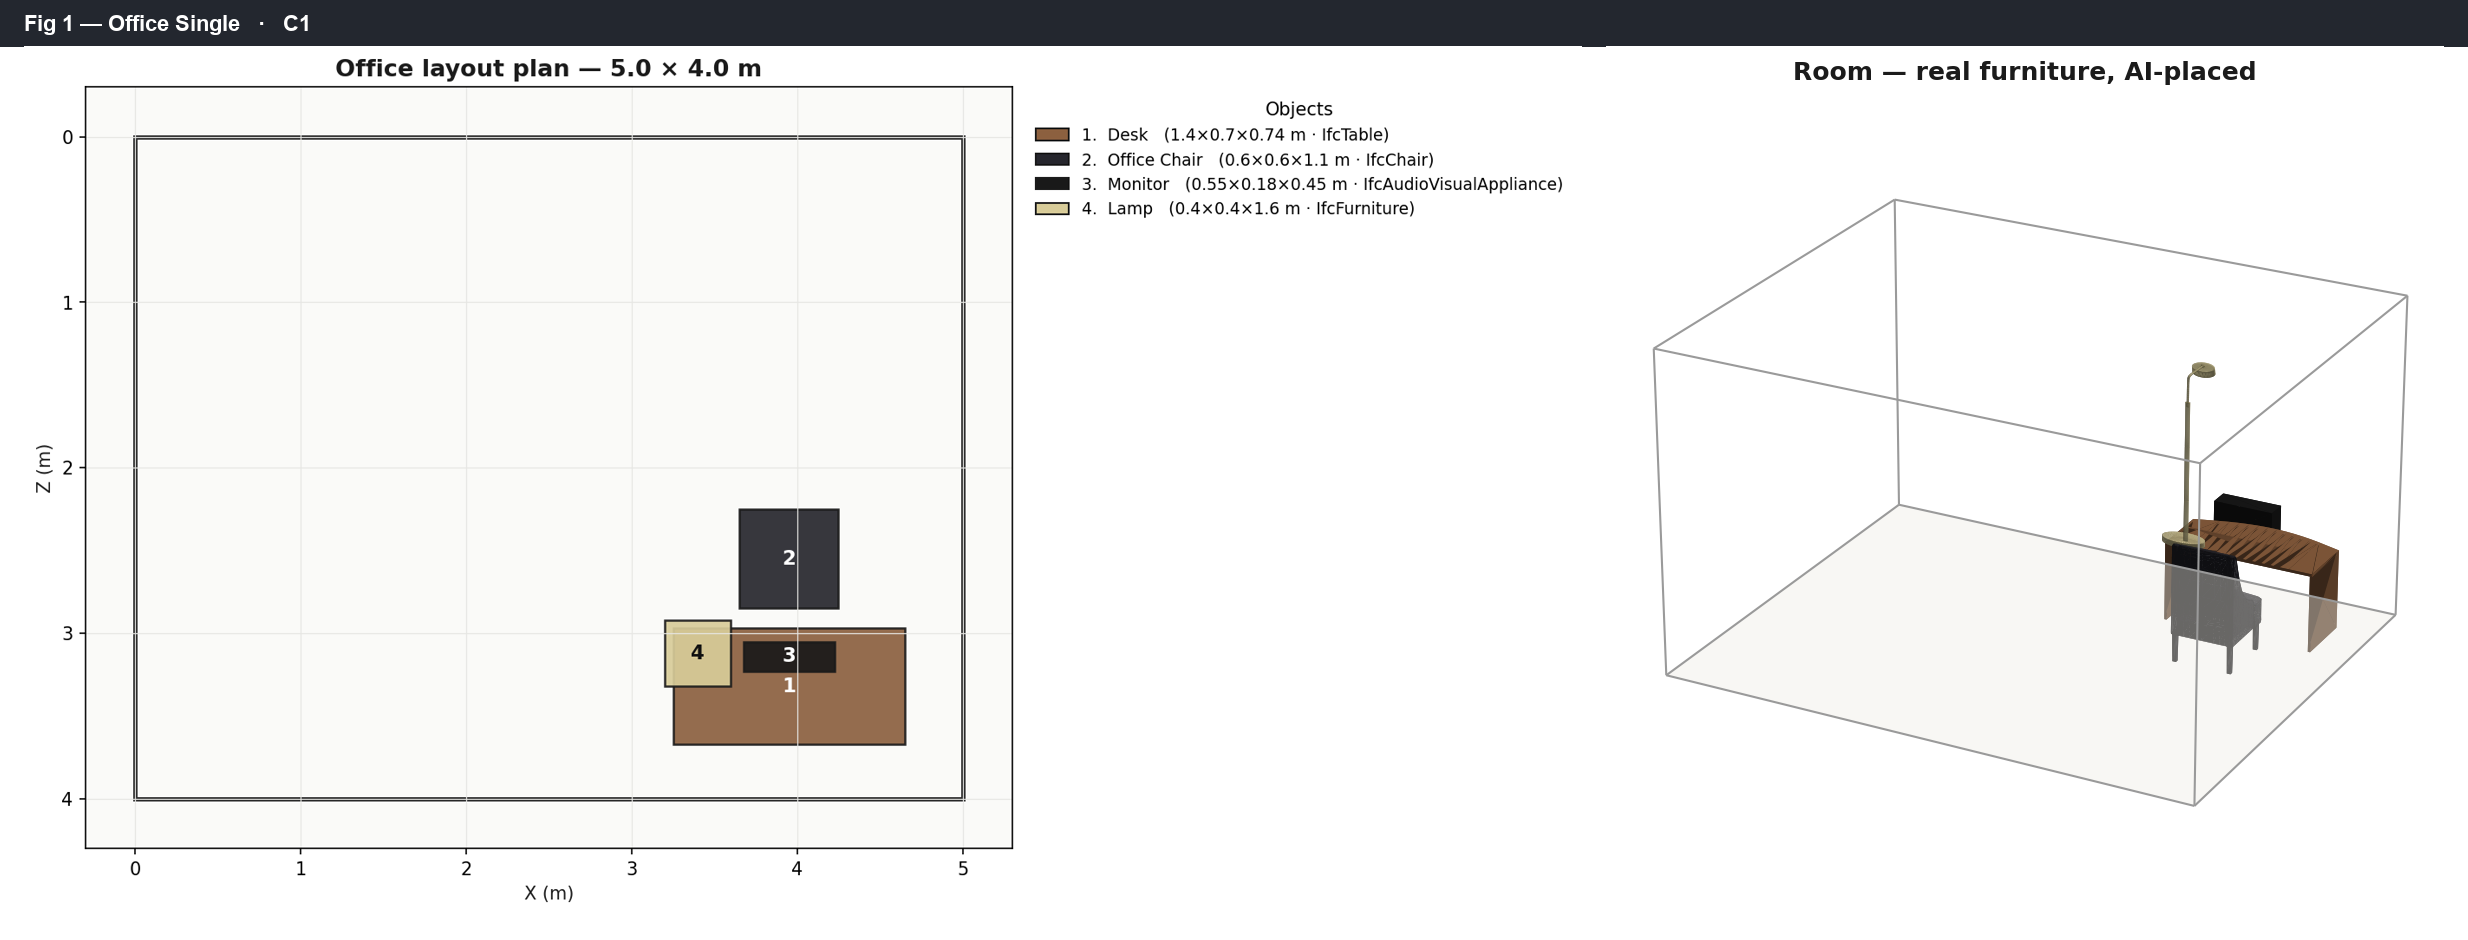
\includegraphics[width=\linewidth]{fig01_office_single_montage.png}
  \caption{Single workstation: chair auto-anchored in front of the desk and turned to face it; monitor + lamp placed on the desk surface. (\textbf{C1}; 5$\times$4~m office, 4 objects, solver: ortools-cpsat).}
  \label{fig:fig01_office_single}
\end{figure}

\begin{figure}[t]
  \centering
  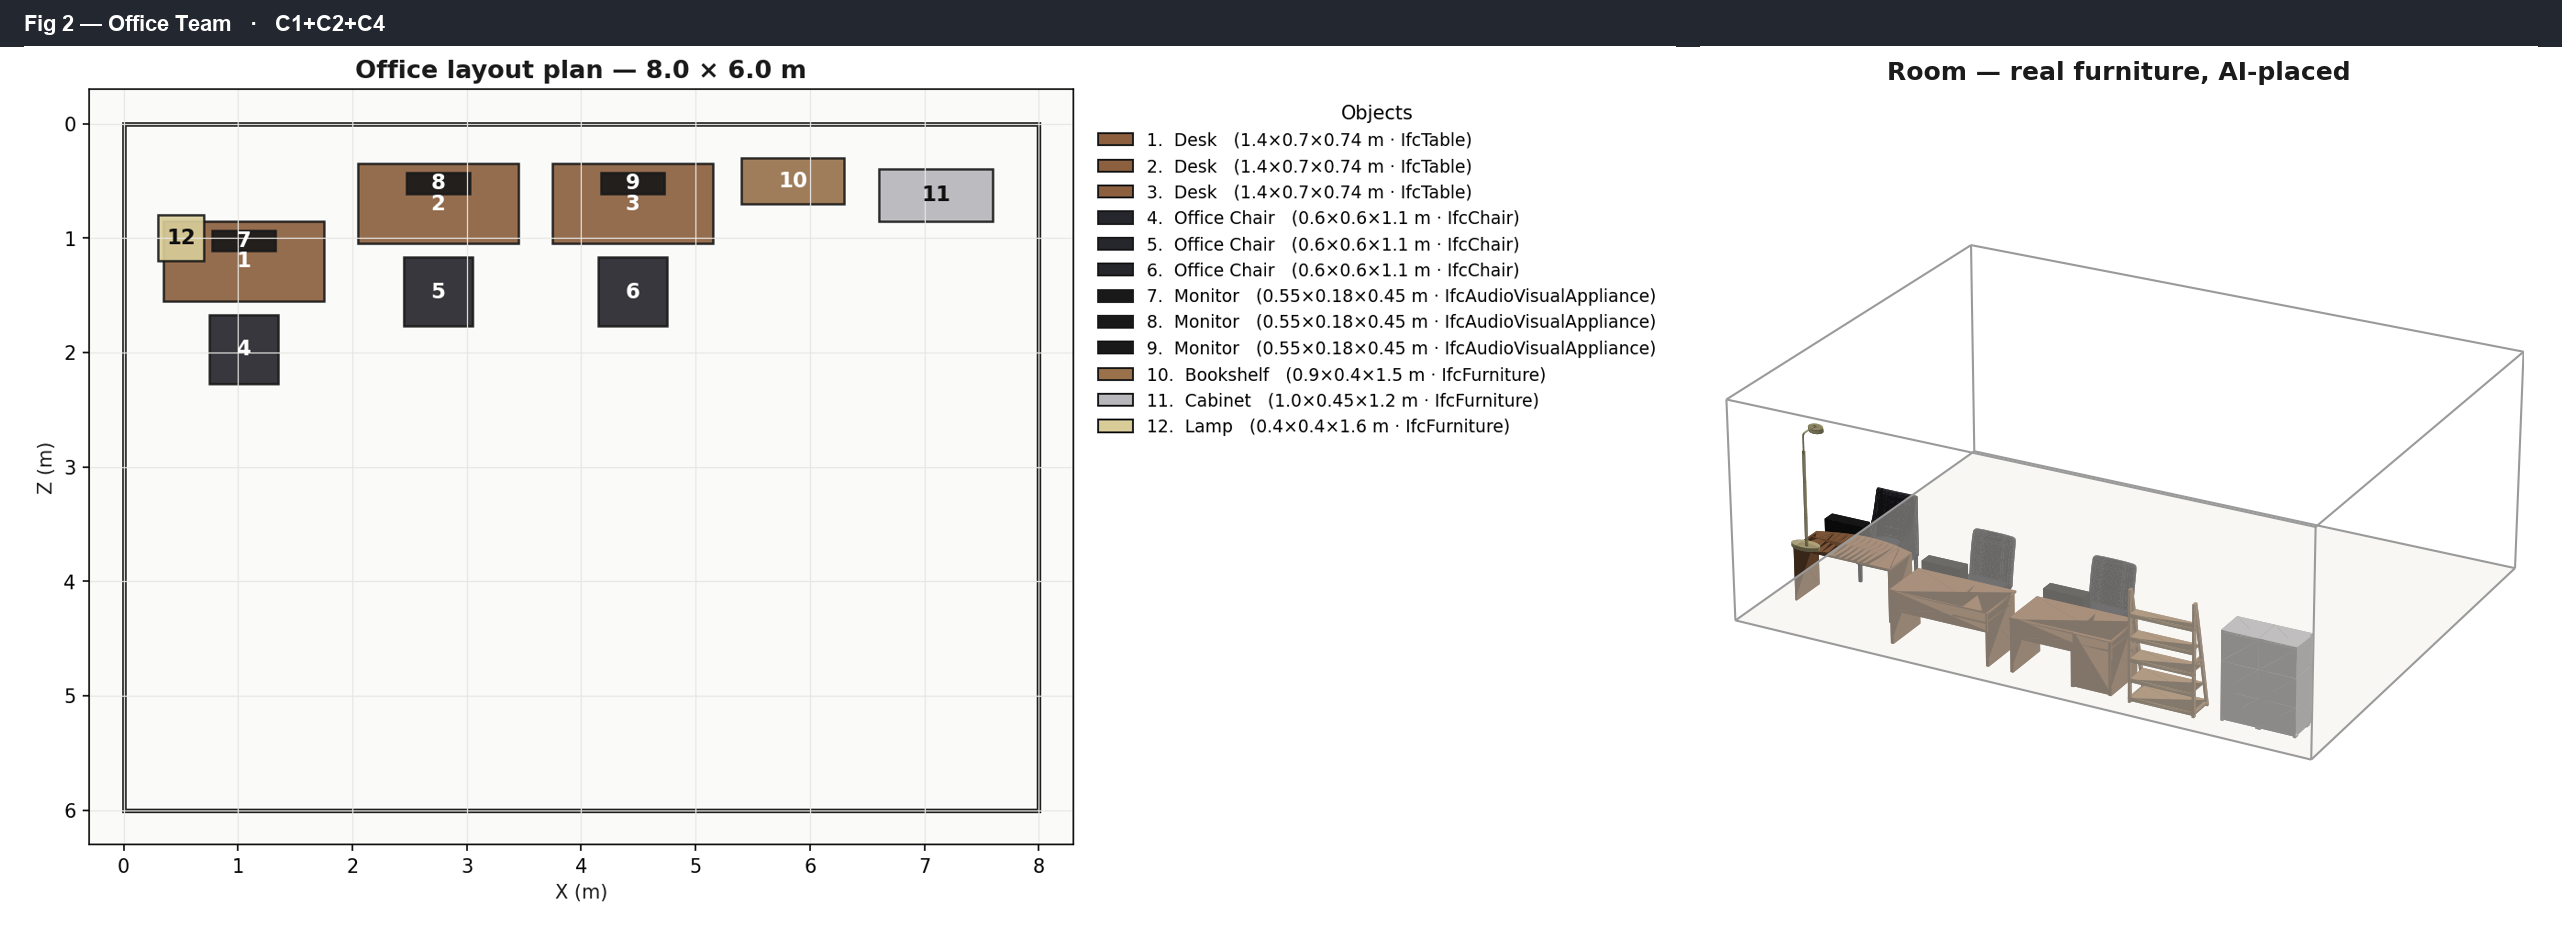
\includegraphics[width=\linewidth]{fig02_office_team_montage.png}
  \caption{Three-workstation office: each desk gets a facing chair + monitor; storage (bookshelf, cabinet) hugs the walls and the centre stays open for circulation. (\textbf{C1+C2+C4}; 8$\times$6~m office, 12 objects, solver: ortools-cpsat).}
  \label{fig:fig02_office_team}
\end{figure}

\begin{figure}[t]
  \centering
  
\includegraphics[width=\linewidth]{fig03_office_obstacles_montage.png}
  \caption{Same office with a structural column and a door keep-clear zone: no furniture overlaps the obstacle and the door swing stays unblocked. (\textbf{C5}; 8$\times$6~m office, 11 objects, solver: ortools-cpsat).}
  \label{fig:fig03_office_obstacles}
\end{figure}

\begin{figure}[t]
  \centering
  
\includegraphics[width=\linewidth]{fig04_office_ada_montage.png}
  \caption{ADA accessibility mode: wider aisles (>=0.915 m route) and door clearances applied, spreading the same furniture for wheelchair circulation. (\textbf{C6}; 8$\times$6~m office, 10 objects, solver: ortools-cpsat).}
  \label{fig:fig04_office_ada}
\end{figure}

\begin{figure}[t]
  \centering
  
\includegraphics[width=\linewidth]{fig05_living_room_montage.png}
  \caption{Living-room rule pack: different functional groups (coffee-table in front of sofa, stools beside the coffee-table) and tighter circulation than the office. (\textbf{C3}; 6$\times$5~m living, 6 objects, solver: ortools-cpsat).}
  \label{fig:fig05_living_room}
\end{figure}

\begin{figure}[t]
  \centering
  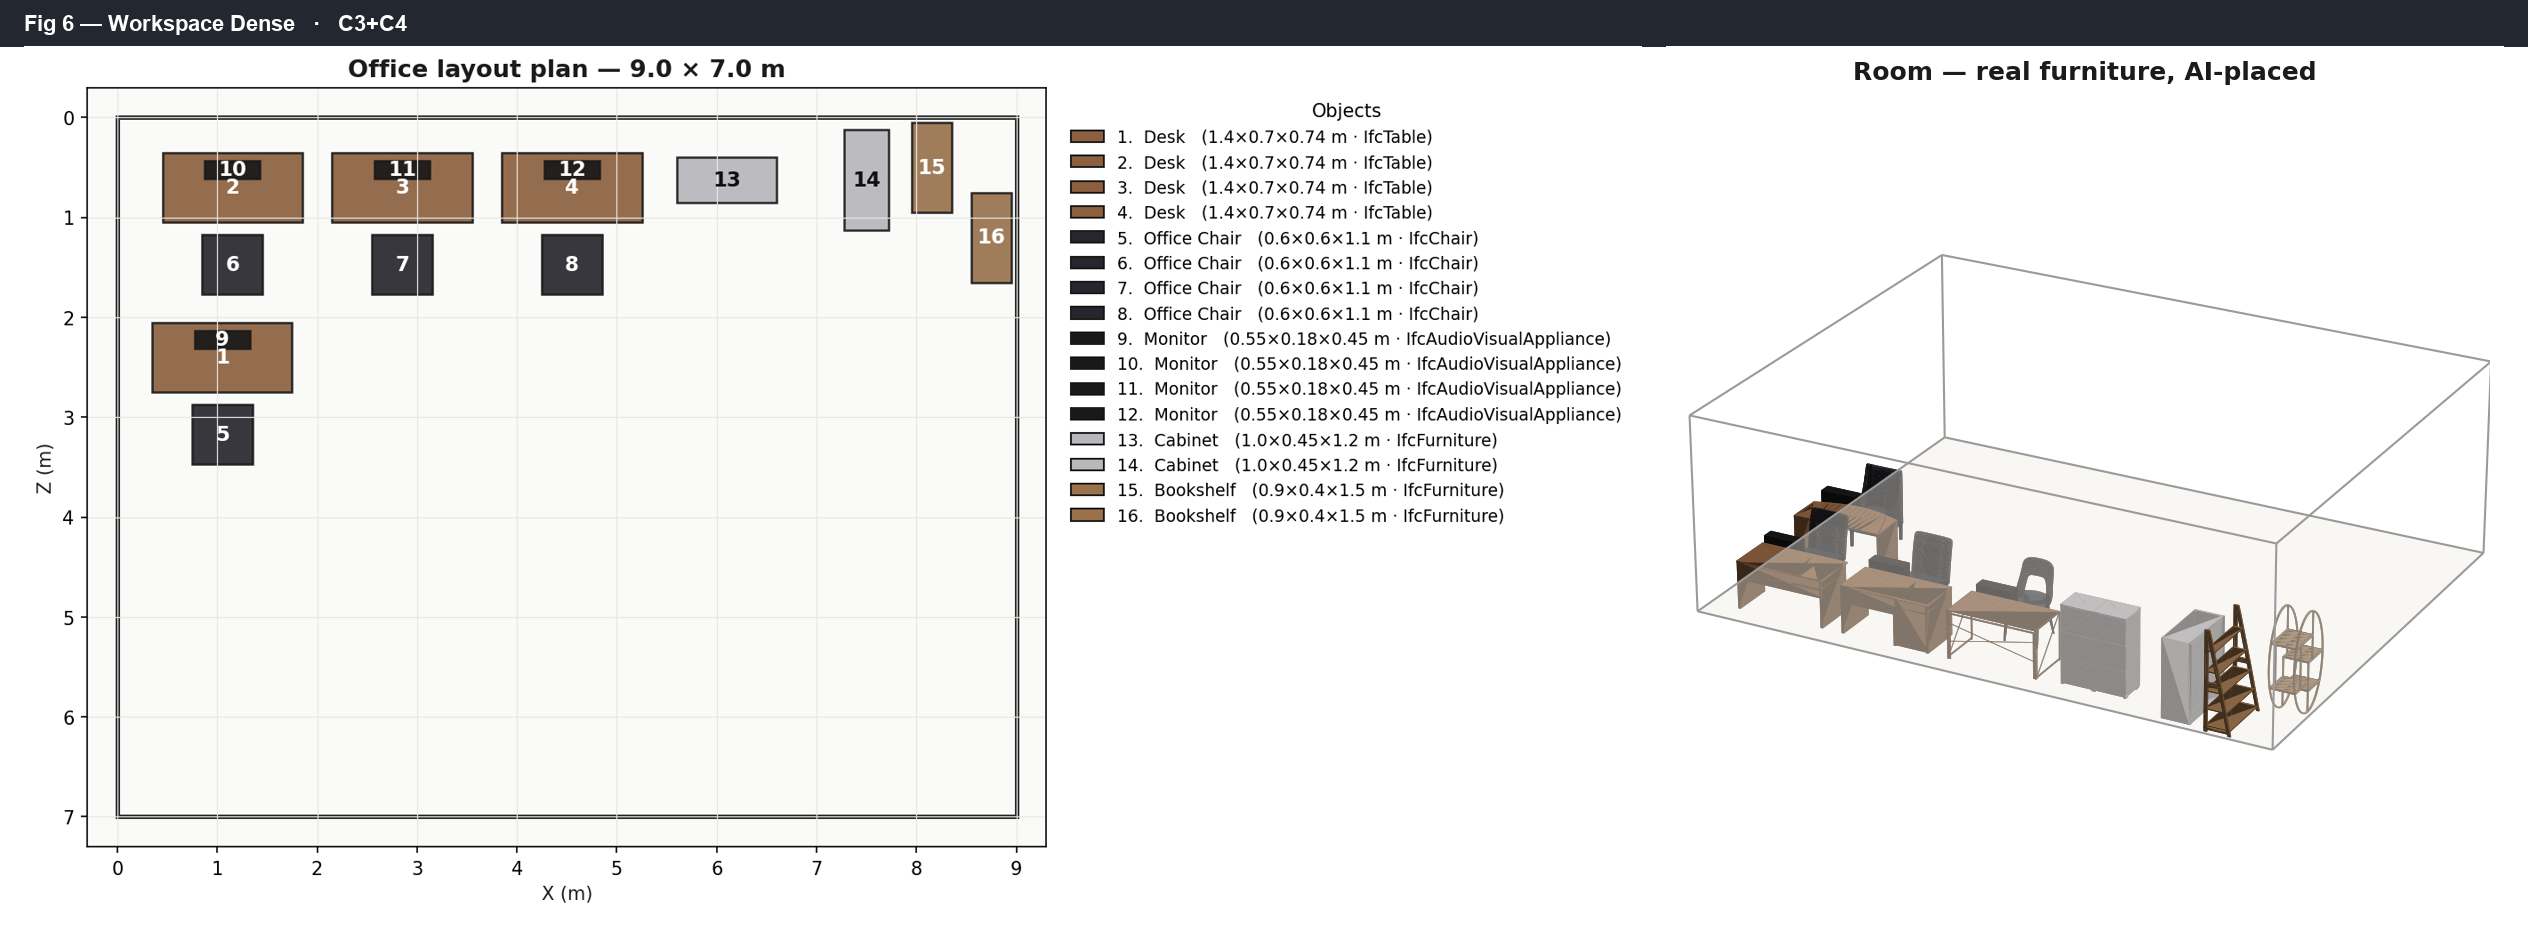
\includegraphics[width=\linewidth]{fig06_workspace_dense_montage.png}
  \caption{Workspace variant (heavier storage, wider aisles) at higher density: four workstations plus storage, testing how the solver scales. (\textbf{C3+C4}; 9$\times$7~m workspace, 16 objects, solver: ortools-cpsat).}
  \label{fig:fig06_workspace_dense}
\end{figure}

\begin{figure}[t]
  \centering
  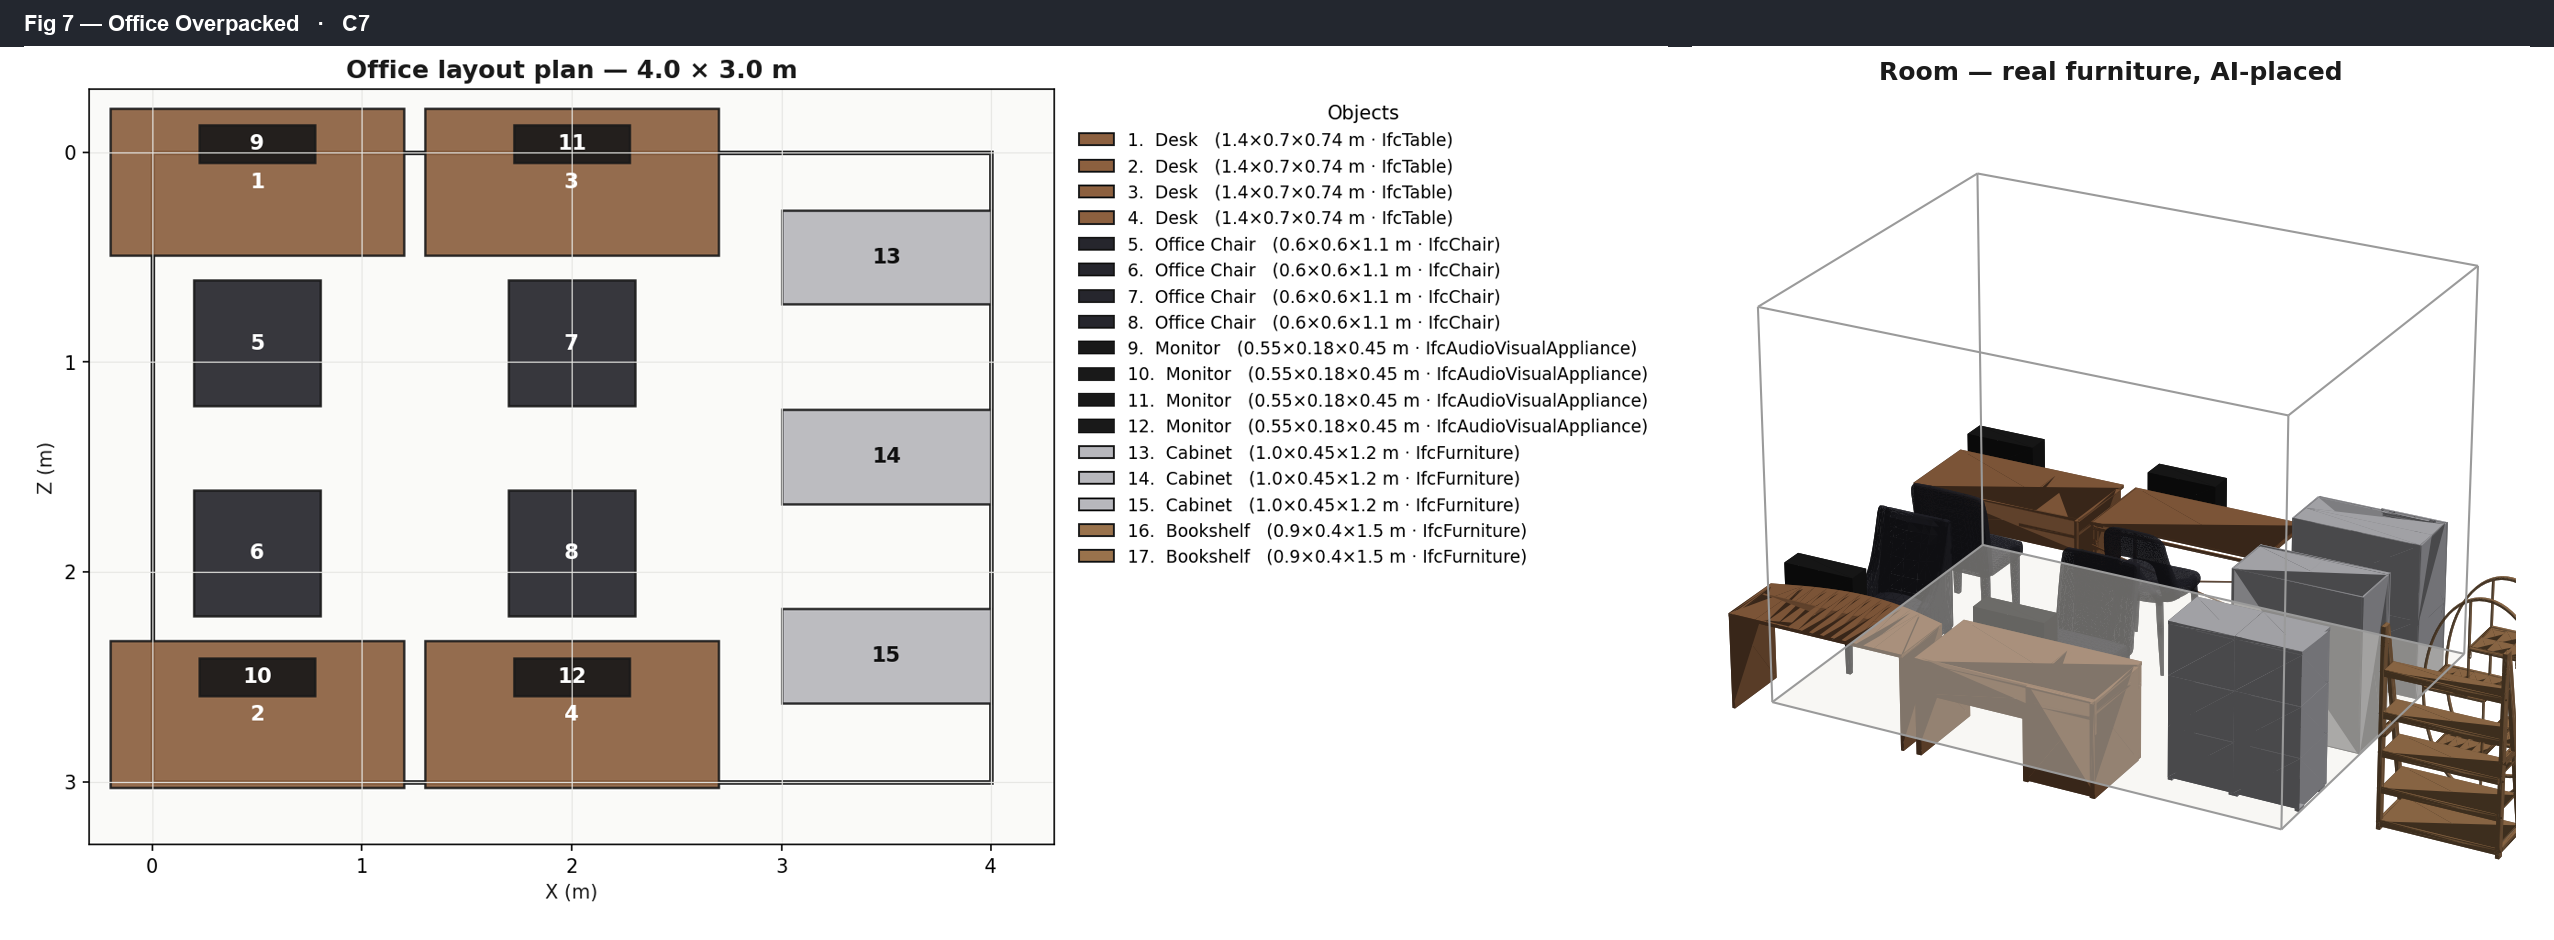
\includegraphics[width=\linewidth]{fig07_office_overpacked_montage.png}
  \caption{Feasibility boundary: deliberately overpacked small room. The solver reports infeasible rather than producing an overlapping (invalid) layout. (\textbf{C7}; 4$\times$3~m office, 17 objects, solver: infeasible-overpacked).}
  \label{fig:fig07_office_overpacked}
\end{figure}

\begin{figure}[t]
  \centering
  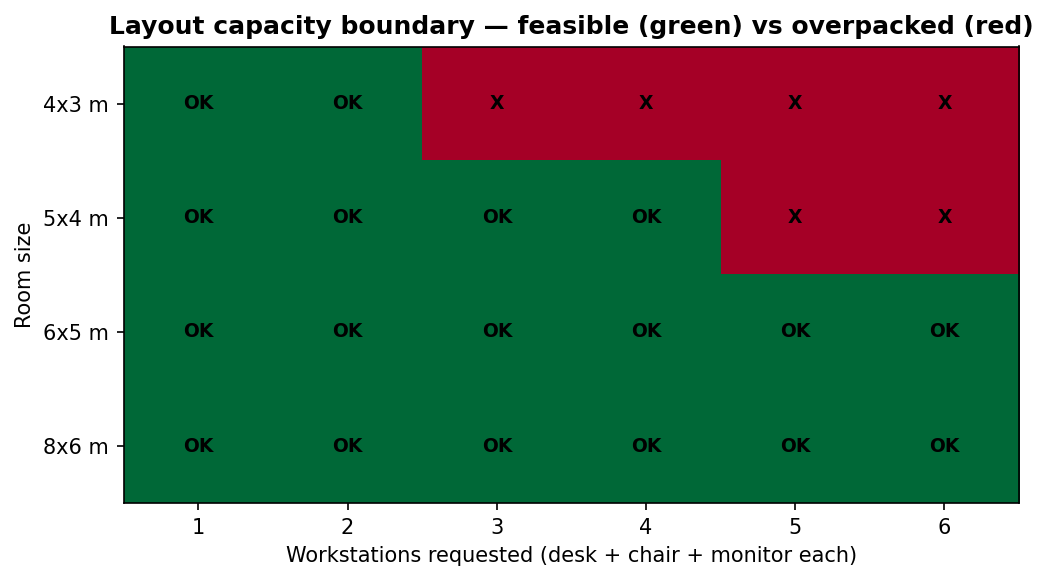
\includegraphics[width=0.8\linewidth]{fig08_capacity_sweep.png}
  \caption{Capacity boundary: for each room size, the largest number of full workstations the solver can place before it reports infeasible.}
  \label{fig:fig08_capacity_sweep}
\end{figure}

\begin{figure}[t]
  \centering
  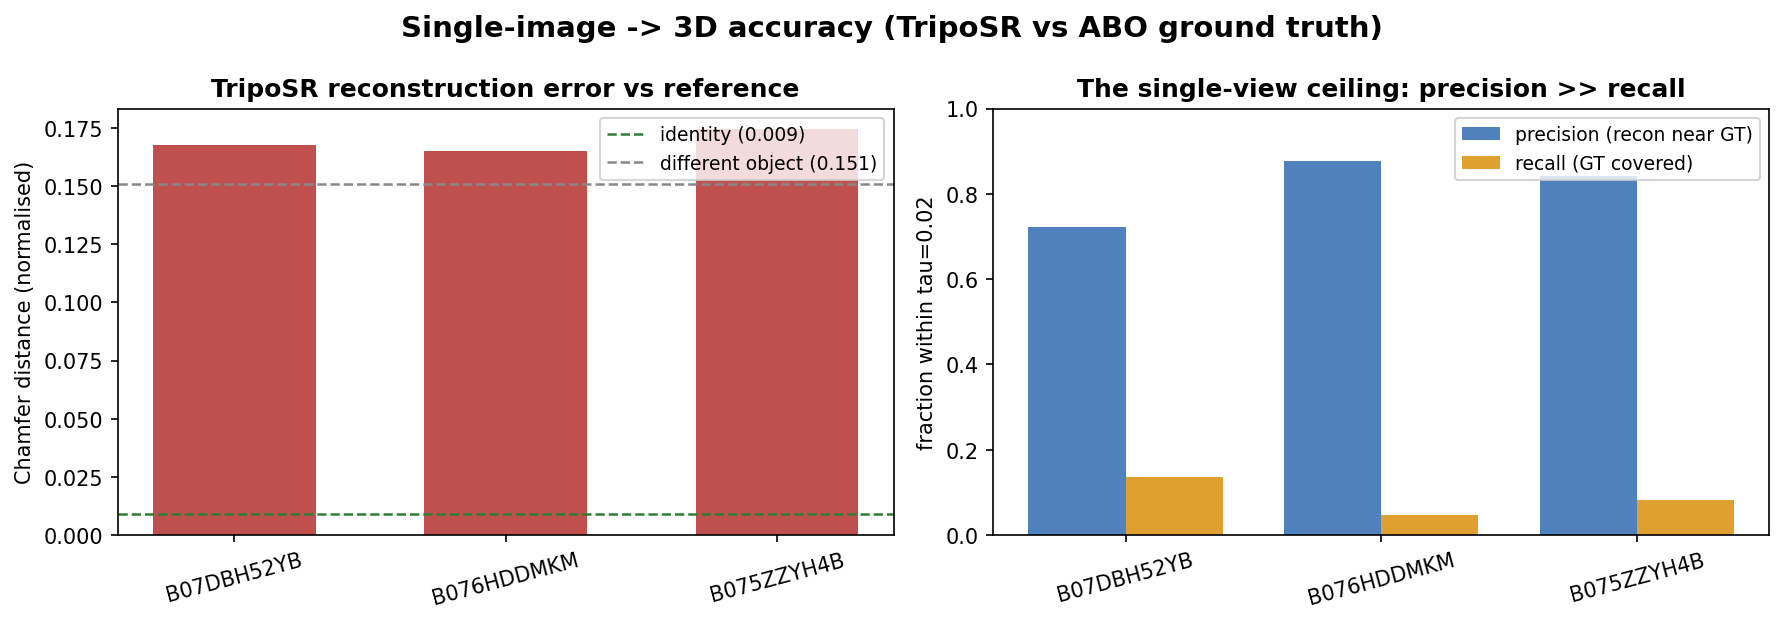
\includegraphics[width=\linewidth]{fig09_accuracy_triposr.png}
  \caption{Single-image$\rightarrow$3D accuracy (TripoSR vs ABO ground truth). Left:
  per-object Chamfer distance sits near the different-object reference, far above identity.
  Right: precision ($\sim$0.81) $\gg$ recall ($\sim$0.09) --- the single-view ceiling
  (visible surface captured, unseen back missed). Section~7.}
  \label{fig:fig09_accuracy_triposr}
\end{figure}

% Composite results plate (all panels on one page) — use figure* for full width in 2-col layouts
\begin{figure*}[t]
  \centering
  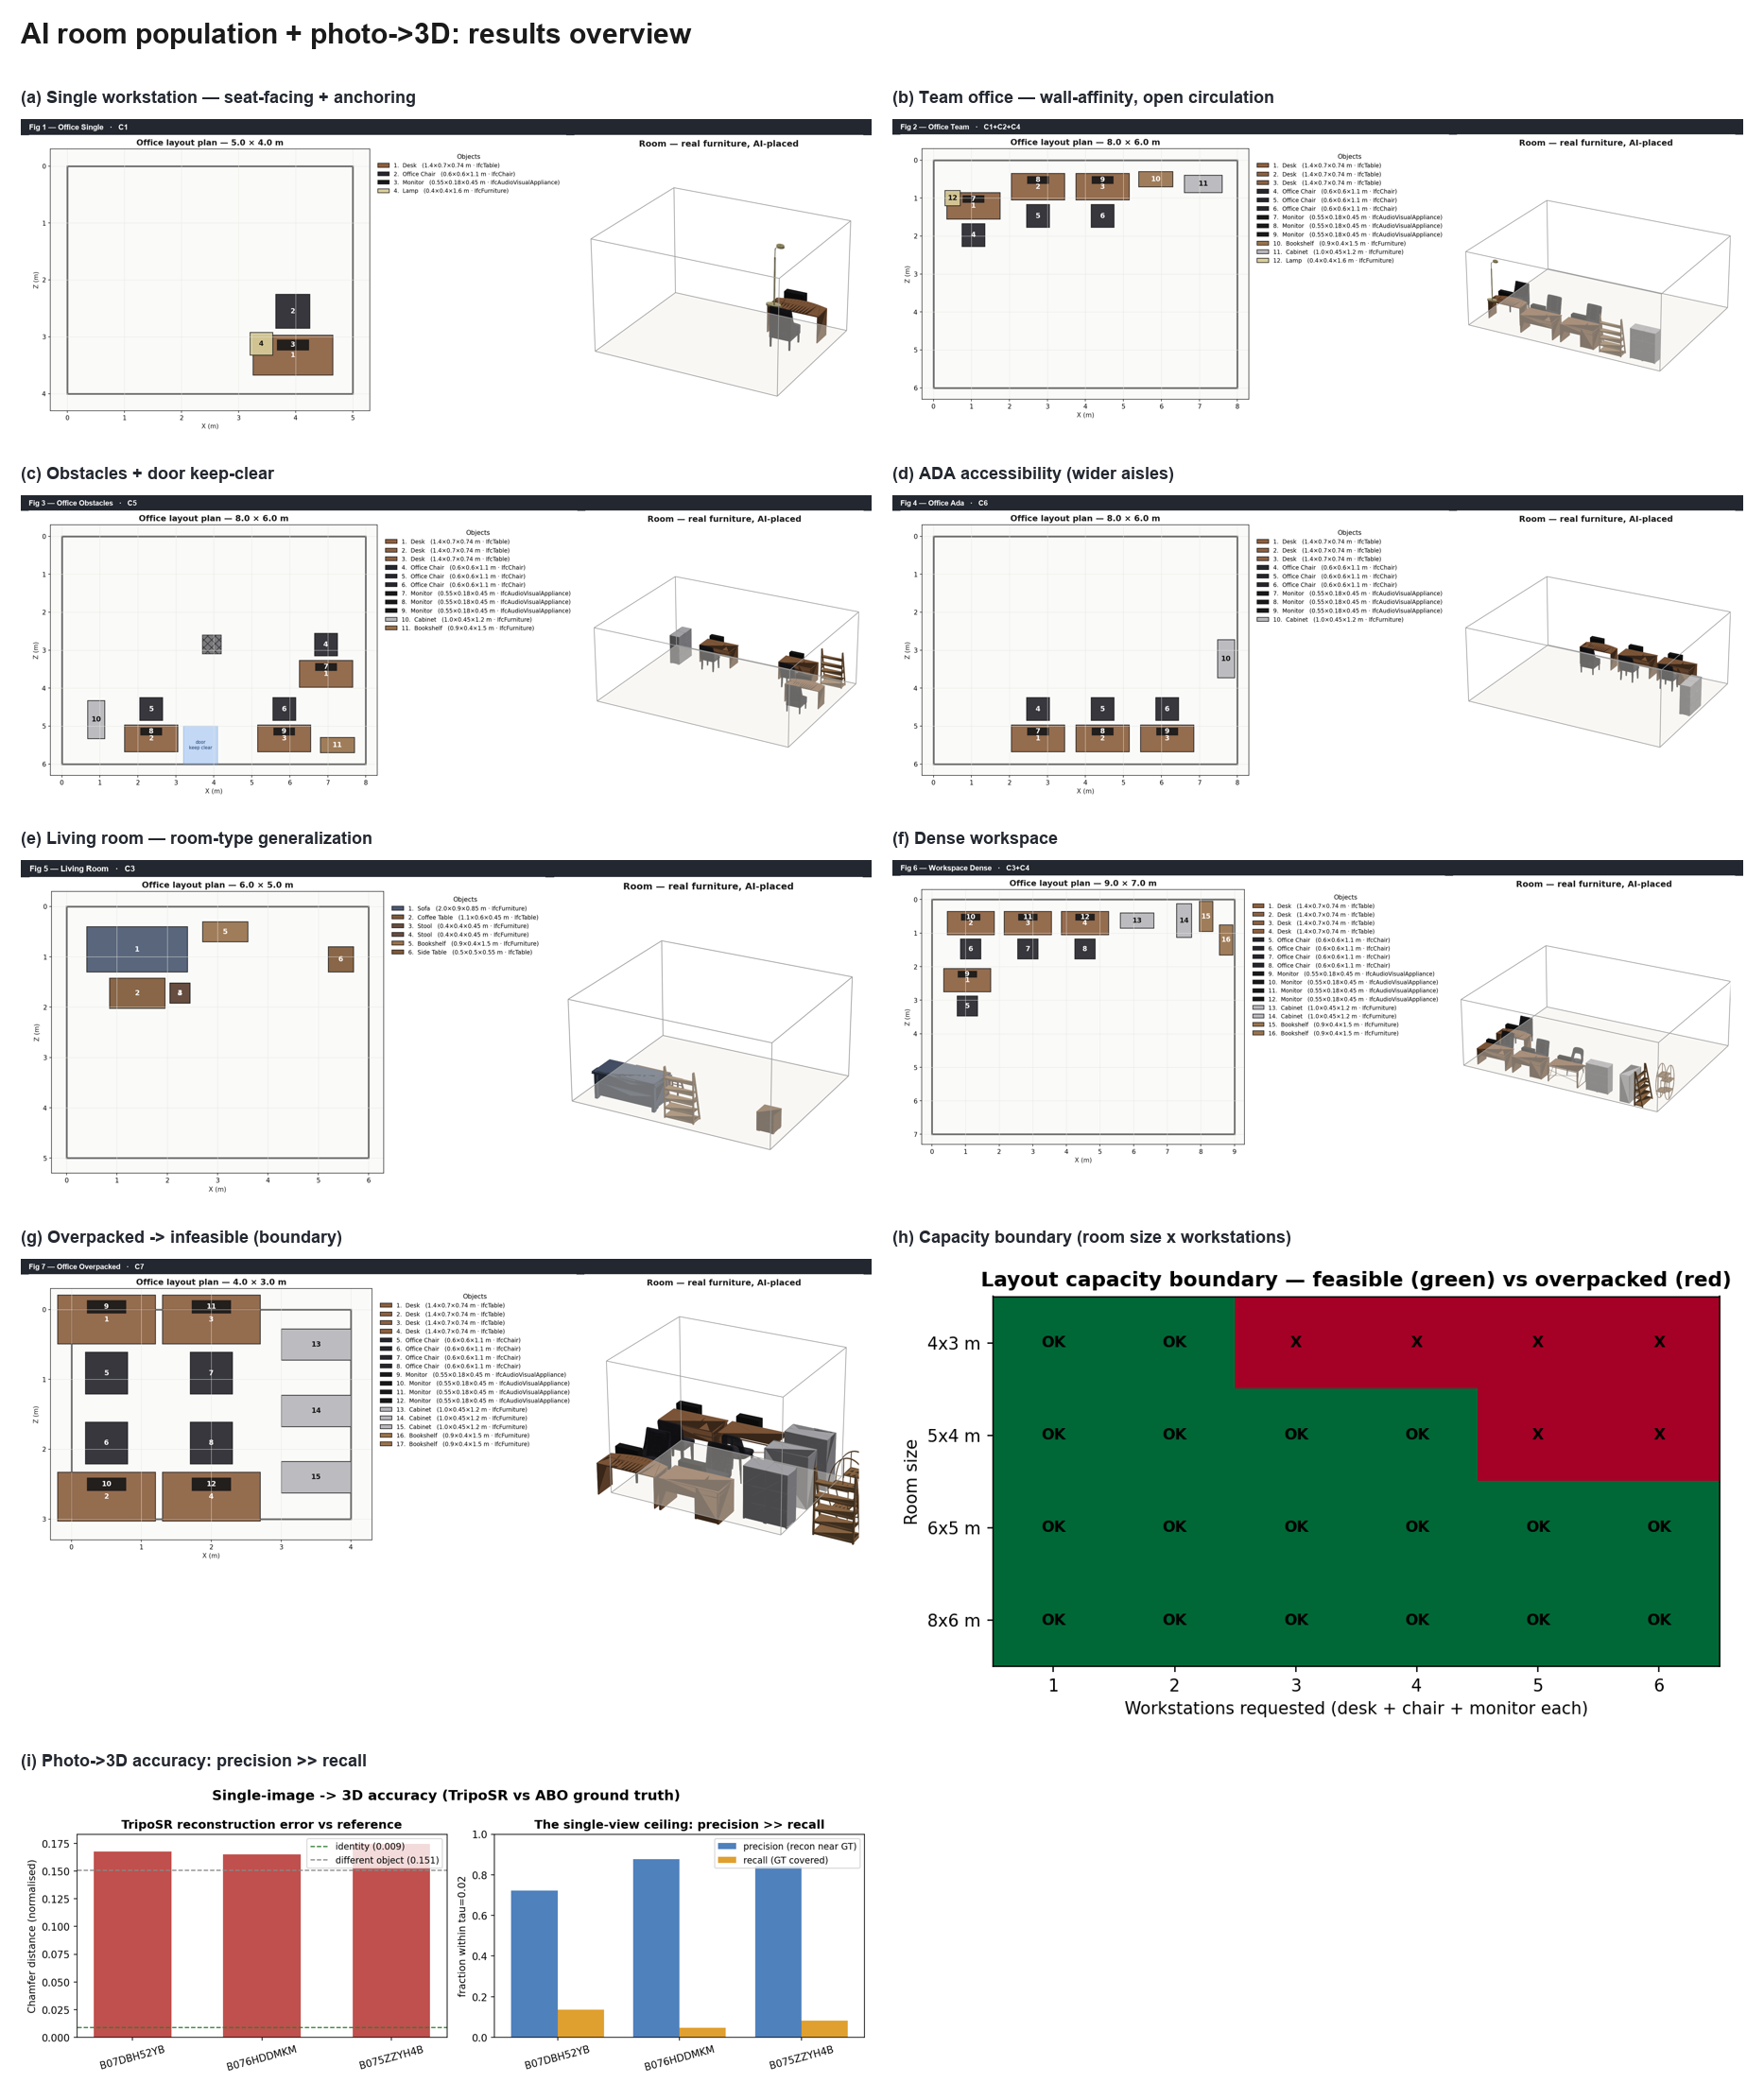
\includegraphics[width=\textwidth]{results_plate.png}
  \caption{Results overview. (a--g) functional room layouts across criteria; (h) capacity
  boundary; (i) photo$\rightarrow$3D accuracy (single-view ceiling). All panels are
  server-side renders generated reproducibly from the pipeline.}
  \label{fig:results_plate}
\end{figure*}
